\documentclass{thesisclass}
% Based on thesisclass.cls of Timo Rohrberg, 2009
% ----------------------------------------------------------------
% Thesis - Main document
% ----------------------------------------------------------------
% No empty in-between chapters, remove this line if desired for double-page printing
\let\cleardoublepage\clearpage

%% -------------------------------
%% |  Information for PDF file   |
%% -------------------------------
\hypersetup{
 pdfauthor={Christian Navolskyi, B. Sc.},
 pdftitle={MIS Compensation: Optimizing Sampling Techniques in Multiple Importance Sampling},
 pdfsubject={Seminar: Advanced Algorithms in Computer Graphics},
 pdfkeywords={MIS}
}


%% ---------------------------------
%% | Information about the thesis  |
%% ---------------------------------

\newcommand{\myname}{Christian Navolskyi, B. Sc.}
\newcommand{\mytitle}{MIS Compensation: Optimizing Sampling Techniques in Multiple Importance Sampling}
\newcommand{\myinstitute}{Institut für Visualisierung und Datenanalyse,\\ Lehrstuhl für Computergrafik}

\newcommand{\reviewerone}{Hisanari Otsu, M. Sc.}
\newcommand{\reviewertwo}{Dr. Christoph Peters}
\newcommand{\advisor}{Hisanari Otsu, M. Sc.}
\newcommand{\advisortwo}{Dr. Christoph Peters}

\newcommand{\timestart}{XX. Monat 20XX}
\newcommand{\timeend}{XX. Monat 20XX}
\newcommand{\submissiontime}{DD. MM. 20XX}


%% ---------------------------------
%% | ToDo Marker - only for draft! |
%% ---------------------------------
% Remove this section for final version!
\setlength{\marginparwidth}{20mm}

\newcommand{\margtodo}
{\marginpar{\textbf{\textcolor{red}{ToDo}}}{}}

\newcommand{\todo}[1]
{{\textbf{\textcolor{red}{(\margtodo{}#1)}}}{}}


%% --------------------------------
%% | Old Marker - only for draft! |
%% --------------------------------
% Remove this section for final version!
\newenvironment{deprecated}
{\begin{color}{gray}}
{\end{color}}


%% --------------------------------
%% | Settings for word separation |
%% --------------------------------
% Help for separation:
% In german package the following hints are additionally available:
% "- = Additional separation
% "| = Suppress ligation and possible separation (e.g. Schaf"|fell)
% "~ = Hyphenation without separation (e.g. bergauf und "~ab)
% "= = Hyphenation with separation before and after
% "" = Separation without a hyphenation (e.g. und/""oder)

% Describe separation hints here:
\hyphenation{
% Pro-to-koll-in-stan-zen
% Ma-na-ge-ment  Netz-werk-ele-men-ten
% Netz-werk Netz-werk-re-ser-vie-rung
% Netz-werk-adap-ter Fein-ju-stier-ung
% Da-ten-strom-spe-zi-fi-ka-tion Pa-ket-rumpf
% Kon-troll-in-stanz
}


%% ------------------------
%% |    Including files   |
%% ------------------------
% Only files listed here will be included!
% Userful command for partially translating the document (for bug-fixing e.g.)
% \includeonly{%
% titlepage,
% contents/
% }


%%%%%%%%%%%%%%%%%%%%%%%%%%%%%%%%%
%% Here, main documents begins %%
%%%%%%%%%%%%%%%%%%%%%%%%%%%%%%%%%
\begin{document}

% Remove the following line for German text
%\selectlanguage{ngerman}

\frontmatter
\pagenumbering{roman}
%% titlepage.tex
%%

% coordinates for the bg shape on the titlepage
\newcommand{\diameter}{20}
\newcommand{\xone}{-15}
\newcommand{\xtwo}{160}
\newcommand{\yone}{15}
\newcommand{\ytwo}{-253}

\begin{titlepage}
% bg shape
\begin{tikzpicture}[overlay]
\draw[color=gray]
 		 (\xone mm, \yone mm)
  -- (\xtwo mm, \yone mm)
 arc (90:0:\diameter pt)
  -- (\xtwo mm + \diameter pt , \ytwo mm)
	-- (\xone mm + \diameter pt , \ytwo mm)
 arc (270:180:\diameter pt)
	-- (\xone mm, \yone mm);
\end{tikzpicture}

\begin{textblock}{10}[0,0](4,2.5)
	
\includegraphics[width=.3\textwidth]{logos/KITLogo_RGB.pdf}
\end{textblock}
\changefont{phv}{m}{n}	% helvetica
\vspace*{3.5cm}
\begin{center}
	\Huge{\mytitle}
	\vspace*{2cm}\\
	\Large{
		Proseminar-Ausarbeitung von
	}\\
	\vspace*{1cm}
	\huge{\myname}\\
	\vspace*{1cm}
	\Large{
		An der Fakultät für Informatik
		\\
		\myinstitute
	}\\
	\vspace*{1cm}
	\Large{\today}
\end{center}
\vspace*{1cm}
%\Large{
%\begin{center}
%\begin{tabular}[ht]{l c l}
%  % Gutachter sind die Professoren, die die Arbeit bewerten.
%  \iflanguage{english}{Reviewer}{Erstgutachter}: & \hfill  & \reviewerone\\
%  \iflanguage{english}{Second reviewer}{Zweitgutachter}: & \hfill  & \reviewertwo\\
%  \iflanguage{english}{Advisor}{Betreuender Mitarbeiter}: & \hfill  & \advisor\\
%  \iflanguage{english}{Second advisor}{Zweiter betreuender Mitarbeiter}: & \hfill  & \advisortwo\\
%  % Der zweite betreuende Mitarbeiter kann weggelassen werden.
%\end{tabular}
%\end{center}
%}


\vspace{2cm}


\begin{textblock}{10}[0,0](4,16.8)
\tiny{
		{KIT -- Universität des Landes Baden-Württemberg und nationales Forschungszentrum der Helmholtz-Gesellschaft}
}
\end{textblock}

\begin{textblock}{10}[0,0](14,16.75)
\large{
	\textbf{www.kit.edu}
}
\end{textblock}

\end{titlepage}

\blankpage


%% -------------------
%% |   Directories   |
%% -------------------
\tableofcontents
\blankpage


%% -----------------
%% |   Main part   |
%% -----------------
\mainmatter
\pagenumbering{arabic}
\chapter{Abstract}
\label{ch:abstract}
Here is some sample text.
\todo{Write abstract (at the end)}
\chapter{Introduction}
\label{ch:introduction}
Since Veach and Guibas introduced Multiple Importance Sampling (MIS)~\cite{veach_guibas}
it had a hugh impact in a variety of directions in computer graphics.
Not only did it help to construct more advanced rendering algorithms like Vertex Connection and Merging~\cite{vcm},
it also helped in calculating direct illumination from area light sources and environment maps~\cite[Chapter~14.3]{pbr-book}
and subsurface scattering~\cite{King}.
Besides being introduced in computer graphics MIS has also been used in other fields~\cite{he}.

For the proof of MIS being almost optimal the assumption was made,
that the distribution of samples among the techniques and the sampling densities are given and fixed.
The only things left for fine tuning was the weighting function
with the balance heuristic being a popular and widely adopted choice because of its simplicity
and proven tight bounds when only using non-negative weights~\cite[Theorem~9.2]{veach-thesis}.
Recently researchers found that using not only non-negative weights can result in a truly optimal weighting function~\cite{Kondapaneni2019}.

No previous work examined the effect of designing a sampling density itself for application in the MIS framework.
Karl\'ik et al. proposed a method to do exactly that and show that it can improve the MIS framework and reduce variance even further.
They assumed multiple sampling techniques and pick one probability density function (pdf) of a technique and modify it in a way that it compensates for the averaging introduced by the balance heuristic.
Their optimization can be applied beforehand and doesn't need adaptive updates as the work of Capp\'e et al.~\cite{Cappe2008}.
Others created product sampling methods~\cite{Herholz} that try to match the integrand closer,
but MIS Compensation as, Karl\'ik et al. call their method,
on the other hand can even cause a pdf to be further away from the integrand but still reduce the variance~\cite{Karlik2019}.



\todo{Write introduction. Structure as in the paper (overview, problem, others, solution proposal)}

\todo{Citation before the dot. In more than one scentance, name in the first sentence and referenc in the last sentence.}
\chapter{Related Work}
\label{ch:related_work}

\textit{Multiple Importance Sampling} The MIS framework was introduced in~\cite{veach_guibas}
and combines multiple different sampling techniques with a weighting function to sample a more complex function better.
In their work they proposed a few different weighting functions the most famous being the balance heuristic,
but also the power and cutoff heuristic which perform better in certain scenarios where one technique matches the integrand well.
Despite the balance heuristic being provably good,
Kondapaneni et al.~\cite{Kondapaneni2019} developed a weighting function that is truly optimal
and uses negative weights to achieve even better results.\\
A lot of work has been put into optimizing the weighting functions,
but Karl\'ik et al. followed a different approach
and worked on a technique to adjust one sampling density to reduce the overall variance.

\textit{Sample distribution} Another direction of research in the field of MIS deals with creating an optimal distribution of the samples over the different sampling techniques.
Pajot et al.~\cite{pajot} proposed a method where they calculate a so called representativity,
based on common rendering information such as the BRDF,
which is a measure of how well a technique matches the integrand.
In a one-sample estimator this representativity can also be used to derive a probability for each sampling strategy.\\
Lu et al.~\cite{lu} created a method where no prior knowledge about the scene is needed to generate a sample distribution over two sampling strategies.
They start by sampling with a small number of samples evenly distributed over the strategies
and calculate a value to partition the total number of samples over the sampling techniques.\\
He and Owen~\cite{he} presented another method to get a partitioning of samples for more than two strategies
by proving that the variance is jointly convex in the distribution of samples.
They also proposed an improved method for convex optimization to find such a distribution.\\
Sbert et al.~\cite{sbert} worked on a modification of the balance heuristic that doesn't take the distribution of samples into account for calculating the weights.
Their method works in two phases.
The first phase uses 20\% of the total samples equally distributed over all sampling methods to calculate the variance $ \sigma^2_i $.
After that the following stage is subdivided into eight substages each using 10\% of the total number of samples
and iteratively updating $ \sigma^2_i $ and calculating the distribution $ \alpha $ over the techniques for the next substage.\\
What all the above techniques have in common is that they all rely on initial samples to fine tune their succeeding execution.
The proposed method of Karl\'ik et al. on the other hand doesn't need any prior samples to be taken and therefore their performance impact should be much smaller~\cite{Karlik2019}.

\textit{Image-based lighting} One widely used application of MIS is image-based lighting with BSDF and HDR map sampling~\cite{pbr-book}.
When using a HDR environment map for direct illumination the pdf for that map is usually proportional to the brightness of the HDR map.
Karl\'ik et al.~\cite{Karlik2019} created a method that alters that sampling density to further decrease the variance.
Agarwal et al.~\cite{agarwal} came up with the idea of stratifying the environment map
and taking into account the visibility in the scene
to create a method that can require up to two orders of magnitude fewer samples for the same quality.\\
Another approach from Clarberg and Akenine-Möller~\cite{clarberg} uses product importance sampling
and creating the BRDF on the fly during rendering.
Their precomputation step uses quadtree-based multiplication while during rendering they build the approximation of the BRDF
and evaluate the product in only one single tree traversal which makes it perform faster than other methods.
The method of Karl\'ik et al.~\cite{Karlik2019} does not change the sampling procedure itself and therefore can work without modifications of the environment map sampler.

\textit{Path guiding} Herholz et al.~\cite{Herholz} worked on a method to create a pdf that resembles the whole product of the integral (BSDF and reflected light) we want to solve,
by training a Gaussian mixture model (GMM) for the individual factors with initial samples,
which they then combine to draw samples during the integration.\\
M\"uller et al.~\cite{mueller2017} also worked on path guiding,
where they used an algorithm that iteratively learns the radiance distribution in the scene to get better samples from their distribution.
The work of Karl\'ik et al.~\cite{Karlik2019} builds on the algorithm proposed by M\"uller et al. to further improve the guiding density.
\chapter{Multiple Importance Sampling}
\label{ch:mis}

\todo{Match to actual structure of this chapter}
In this chapter the fundamentals of Monte Carlo integration and importance sampling will be introduced.
Following that Multiple Importance Sampling is explained which is essential for the next chapter \ref{ch:mis_compensation}.


\section{Probability Basics}
\label{sec:probability_basics}
For our use case we need to define random variables, probability distribution functions (pdf) and cumulative distribution functions (cdf).
A random variable maps an event to a real number $ X: \Omega \to \mathbb{R} $.
In a discrete scenario our random variable corresponds to one exact event e.g. a dice throw showing three pips on the top.
The probability for this can be expressed as $ P(X = 3) = \frac{1}{6} $ or as $ X(3) = \frac{1}{6} $
since the random variable $ X $ can take six different values which are all equally likely.
To express the probability that an event is within a range of values we can use the cdf
which is defined as $$ F(x) = P(X \leq x), x \in \mathbb{R}. $$
For the probability of a random variable in an interval $ [a, b) $ we can write $$ P(a \leq X < b) = F(b) - F(a)~\cite{pris}. $$

When we are talking about continuous events e.g. turning a wheel of fortune, every exact angle has a probability of nearing zero.
But we can still express our probability for an angle interval with the cdf from above.
In the continuous case we have a pdf that is used to calculate the cdf with $$ F(x) = \int_{-\infty}^x p(\tilde{x}) d\tilde{x}. $$
The pdf has to be non-negative ($ \forall x: p(x) \geq 0 $) and integrate to one ($ \int_{-\infty}^{\infty} p(x) dx = 1$) to be valid and
\enquote{[...] describes the relative probability of a random variable taking on a particular value}~\cite[Chapter~13.1]{pbr-book}.
\todo{How to cite when the content of this section was created with a reference?}


\section{Generating Samples after a specific Function}
\label{sec:sample_generation}
This will be essential for the next section \ref{sec:monte_carlo},
since this is our adjustment wheel to manipulate the quality of our rendering (for a given amount of time).
Most of the time we don't need evenly distributed samples,
rather our samples should follow a specific characteristic of a material or a scene.
For this we need to know how to generate samples that correspond to that characteristic.

Given a function $ f(x) $ from which we would like to draw samples from the first step is to make sure
it fulfills the constraints for a pdf in an interval $ [a, b) $ we want to use.
First we check that $ \forall x \in [a, b): f(x) \geq 0 $ and then calculate the integral with
\begin{equation}
\label{eq:integral_fx}
    F = \int_{a}^b f(x) dx.
\end{equation}
$ F $ can be used to normalize our goal function which yields us $ \tilde{f}(x) = \frac{f(x)}{F} $ as a valid pdf.
The next step is to calculate our cdf as $ F(x) = \int_{a}^x \tilde{f}(t) dt $ which we will then invert to get $ F^{-1}(x) $.
Now we only need to draw an equally distributed random number (which most programming languages have a library for) in the interval $ [0, 1) $
which we call $ \xi $ and evaluate $ F^{-1}(\xi) = X $ to get $ X $ which is distributed proportional to $ f(.) $.
This method is called "inverse cdf"~\cite{pris}.
\todo{Should I also cover 2D sampling?}
\todo{Should I cover more sampling methods (rejection sampling e.g.)}


\section{Monte Carlo Integration}
\label{sec:monte_carlo}
Monte Carlo integration is a technique to approximate the integral of an arbitrary function $ f(x) $
by taking $ N $ random samples $ X_i $ from a pdf $ p(X_i) $.
As we know the expectation of a random variable is calculated by $$ E(X) = \int_{-\infty}^\infty x p(x) dx $$
or more generally $$ E(g(x)) = \int_{-\infty}^\infty g(x) p(x) dx. $$
For the next step we need the law of large numbers which states that $$ P\left[ \lim_{N\to\infty} \frac{1}{N} \sum_{i = 1}^N X_i = E(X) \right] = 1 $$
with $ X_i $ drawn from $ p(.) $ which means that the average of our samples will converge to the expected value~\cite[Chapter~2.4.1]{veach-thesis}.
From here we can formulate
\begin{equation*}
    \int_{a}^b g(x) p(x) dx \stackrel{definition}{=} E(g(x))
    \stackrel{law~of~large~numbers}{\approx} \frac{1}{N} \sum_{i = 1}^N g(x_i)
\end{equation*}
and with $ g(x) = \frac{f(x)}{p(x)} $
\begin{equation}
\label{eq:monte_carlo_integral}
\begin{aligned}
    \int_{a}^b \frac{f(x)}{p(x)} p(x) dx &\approx \frac{1}{N} \sum_{i = 1}^N \frac{f(x)}{p(x)} \\
    \Leftrightarrow \int_{a}^b f(x) dx &\approx \frac{1}{N} \sum_{i = 1}^N \frac{f(x)}{p(x)}
\end{aligned}
\end{equation}
which is the Monte Carlo estimator~\cite{pris}.


\subsection{Variance}
\label{sec:variance}
Generally the variance is described by $$ V(X) = \frac{1}{N} \sum_{i = 1}^N (x_i - E(X))^2 $$ for discrete random variables~\cite{pris}
and $$ V(X) = \int_{a}^b (x - I)^2 p(x) dx $$ with $ I $ being the mean of the random variable $ X $ for continuous variables~\cite{wyzant}.
When we look at the variance of our Monte Carlo integral we get
\begin{equation}
\label{eq:monte_carlo_variance}
\begin{aligned}
    V(g(x)) &= \int_{a}^b (g(x) - F)^2 p(x) dx \\
            &= \int_{a}^b \left(\frac{f(x)}{p(x)} - F\right)^2 p(x) dx
\end{aligned}
\end{equation}
with $ F $ being the integral from equation \ref{eq:integral_fx}.


\section{Importance Sampling}
\label{sec:importance_sampling}
With the variance from equation \ref{eq:monte_carlo_variance} let's see how we can improve it.
We can easily see that reducing the term $ \frac{f(x)}{p(x)} - F $ will finally reduce the variance the most since it will be exponentiated.
Since $ F $ and $ f(.) $ are fixed (that is the integral we want to calculate) only $ p(.) $ is left for modification.
When we choose $$ p(x) = \frac{f(x)}{\int_{a}^b f(x) dx} $$ we get
\begin{equation*}
\begin{aligned}
    \frac{f(x)}{p(x)} - F &= \frac{f(x)}{f(x)}\int_{a}^b f(x) dx - F \\
        &\stackrel{\ref{eq:integral_fx}}{=} \int_{a}^b f(x) dx - \int_{a}^b f(x) dx
        &= 0
\end{aligned}
\end{equation*}
which is ideal as we get a variance of 0 and are done.
The problem is that we don't know the integral at the start since that is what we want to calculate in the first place.
When we look at our chosen pdf we see that $ p(.) $ is proportional to $ f(.) $ by a factor $ \frac{1}{\int_{a}^b f(x) dx} = \frac{1}{F} := c $.
So we should at least try to chose $ p(.) $ somewhat proportional to $ f(.) $.
The difficulty is that $ f(.) $ can be arbitrary complex so we might only be able to approximate some part of it with one specific pdf.


\section{Multiple Importance Sampling}
\label{sec:multiple_importance_sampling}
The rendering equation
\begin{equation}
    \label{eq:rendering_equation}
    L_o(x, \omega) = L_e(x, \omega) + \int_{\Omega^+} f_s(x, \omega, \omega_o) L_r(x, \omega_o) |n \cdot \omega_o|^+ d\omega_o
\end{equation}
consists of the emitted light at point $ x $ $ L_e(.) $,
the bidirectional scattering distribution function (BSDF) $ f_s(.) $,
the reflected light at point $ x $ in direction $ \omega $ expressed as $ L_r(.) $
and the cosine to account for looking at an angle onto the surface $ |n \cdot \omega_o|^+ $
where the $ ^+ $ means we are only taking values $ > 0 $ so only directions pointing into the upper hemisphere.
With this we can see that a single pdf that only is proportional to e.g., the BSDF leaves out the $ L_r(.) $ term so it can't be optimal.
Having multiple pdfs where each samples a different part of the rendering equation well
a combination of them should create a good result.
E. Veach created a good example of this problem in his thesis~\cite{veach-thesis} which can be seen in figure \ref{fig:veach_mis_single}.
He also introduced Multiple Importance Sampling to use a combination of pdfs to get better results than would be possible with only one pdf.

When sampling only the BSDF we see that in figure \ref{fig:veach_mis_bsdf} the bottom left reflection is very noisy,
because sampling a diffuse BSDF can give a wide range of directions
and since the light source on the left is very small only very few directions will point directly on that light source.
The more specular surfaces in that figure are well sampled which makes sense,
because there are less possible directions to sample so the reflection will be well sampled.

On the other hand figure \ref{fig:veach_mis_light} shows the same scene but sampled after the light sources
by sampling a random point on the light source and then evaluating the render equation to get the contribution.
Here the opposite happened in the two corners we looked at before.
The bottom left reflection is very well sampled
since the direction to the light source is still valid (has some contribution in the BSDF) and therefore we can see the whole reflection.
But now the top right reflection is noisy because the direction to a random point on the light source has no contribution in the BSDF.

\begin{figure}
    \centering
    \begin{subfigure}[b]{0.45\textwidth}
        \centering
        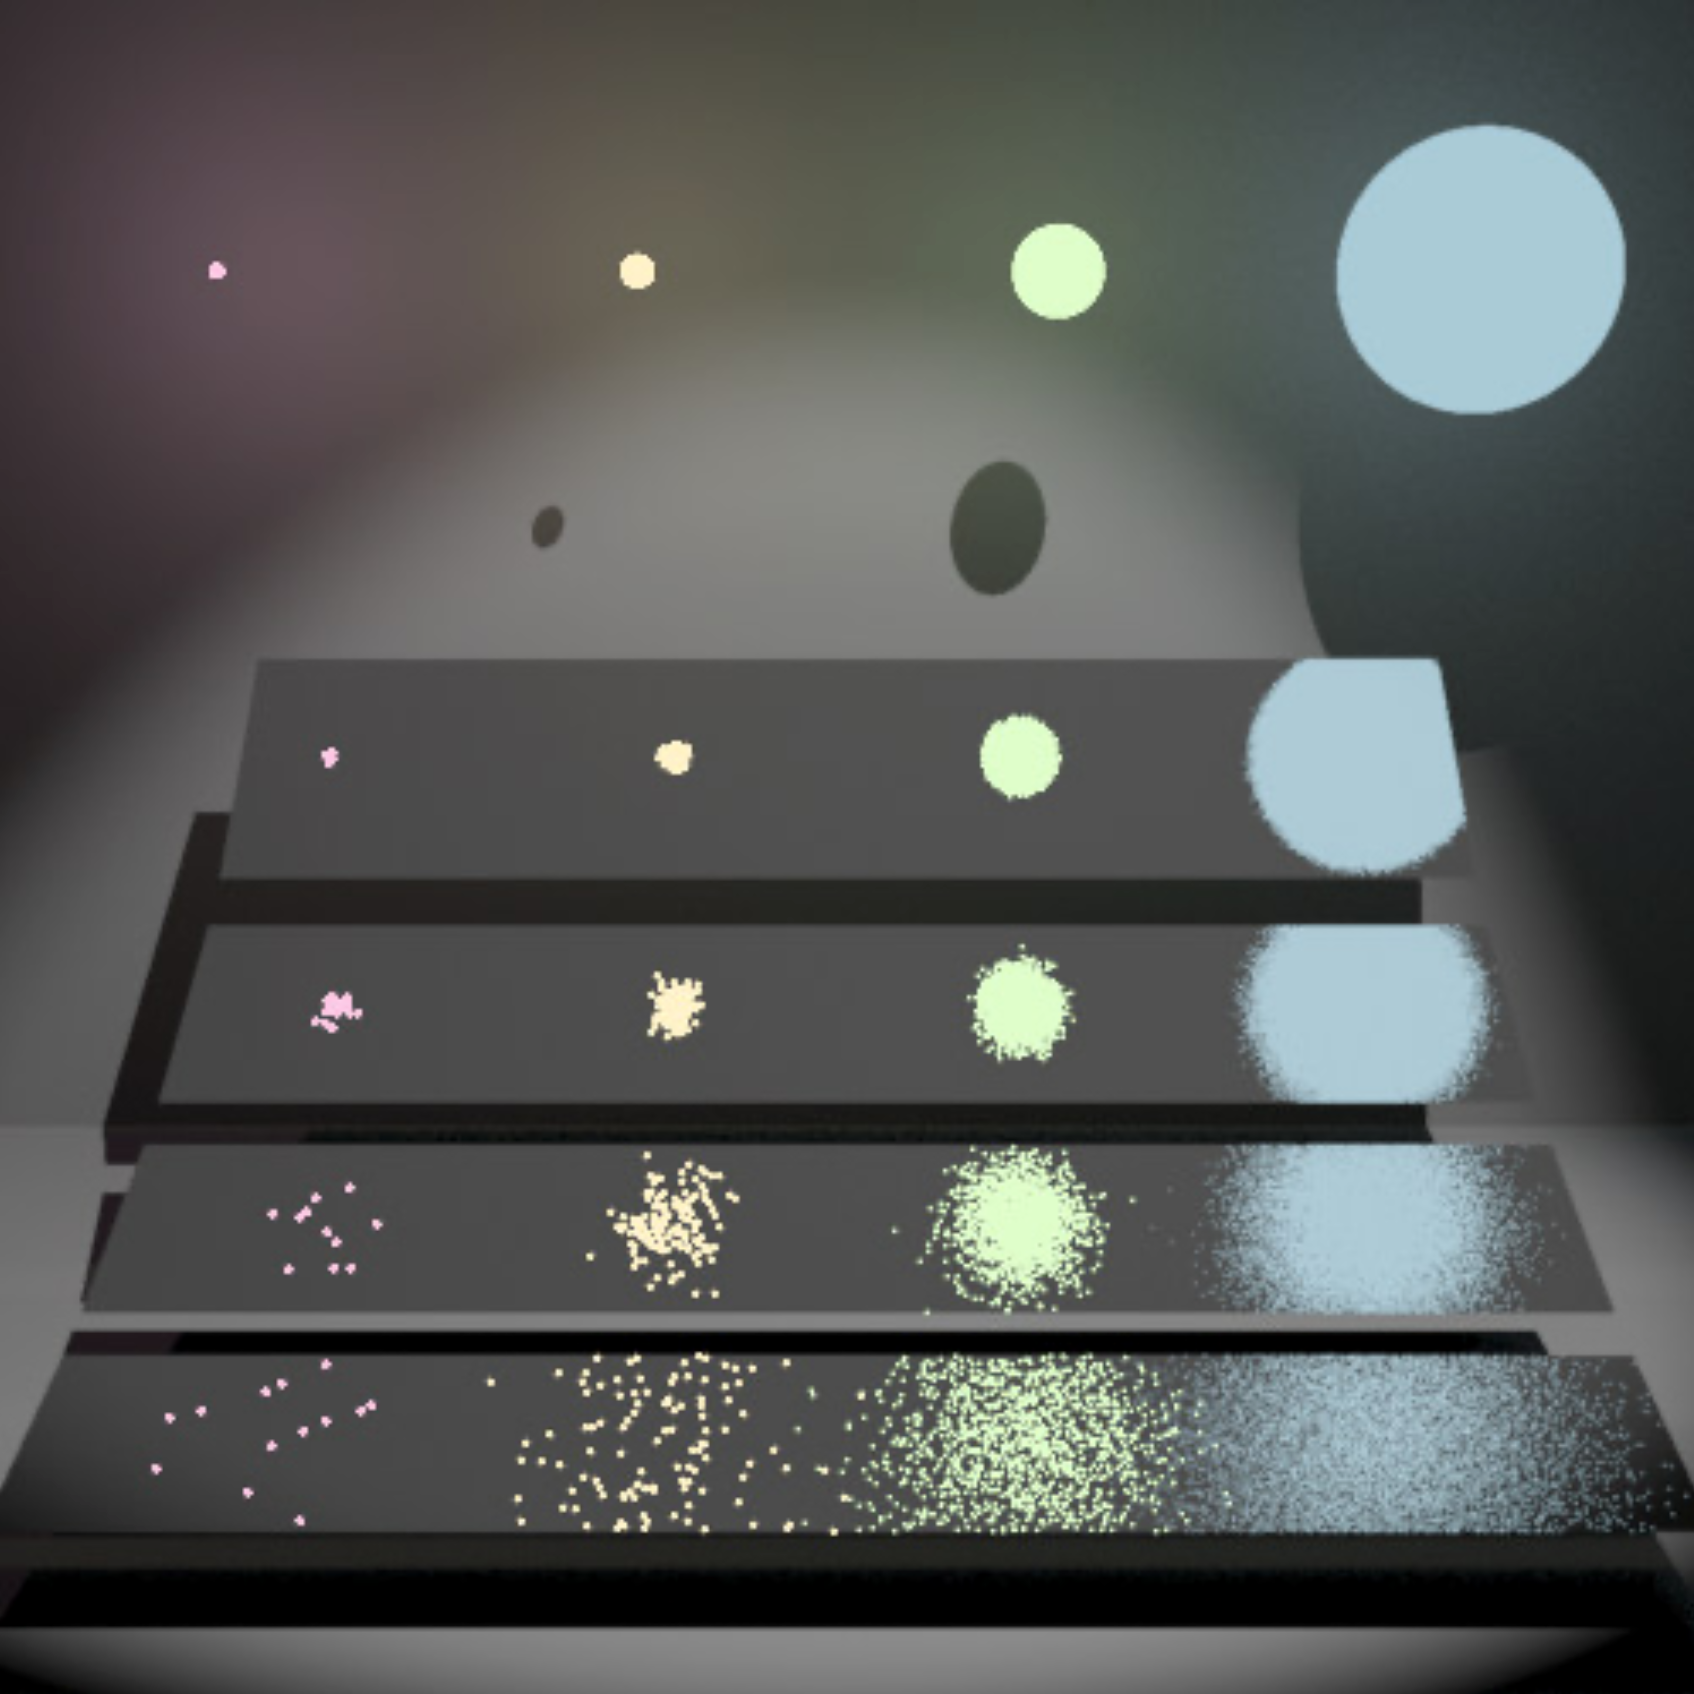
\includegraphics[width=\textwidth]{images/veach_mis_bsdf.png}
        \caption{Sampled after the BSDF}
        \label{fig:veach_mis_bsdf}
    \end{subfigure}
    \hfill
    \begin{subfigure}[b]{0.45\textwidth}
        \centering
        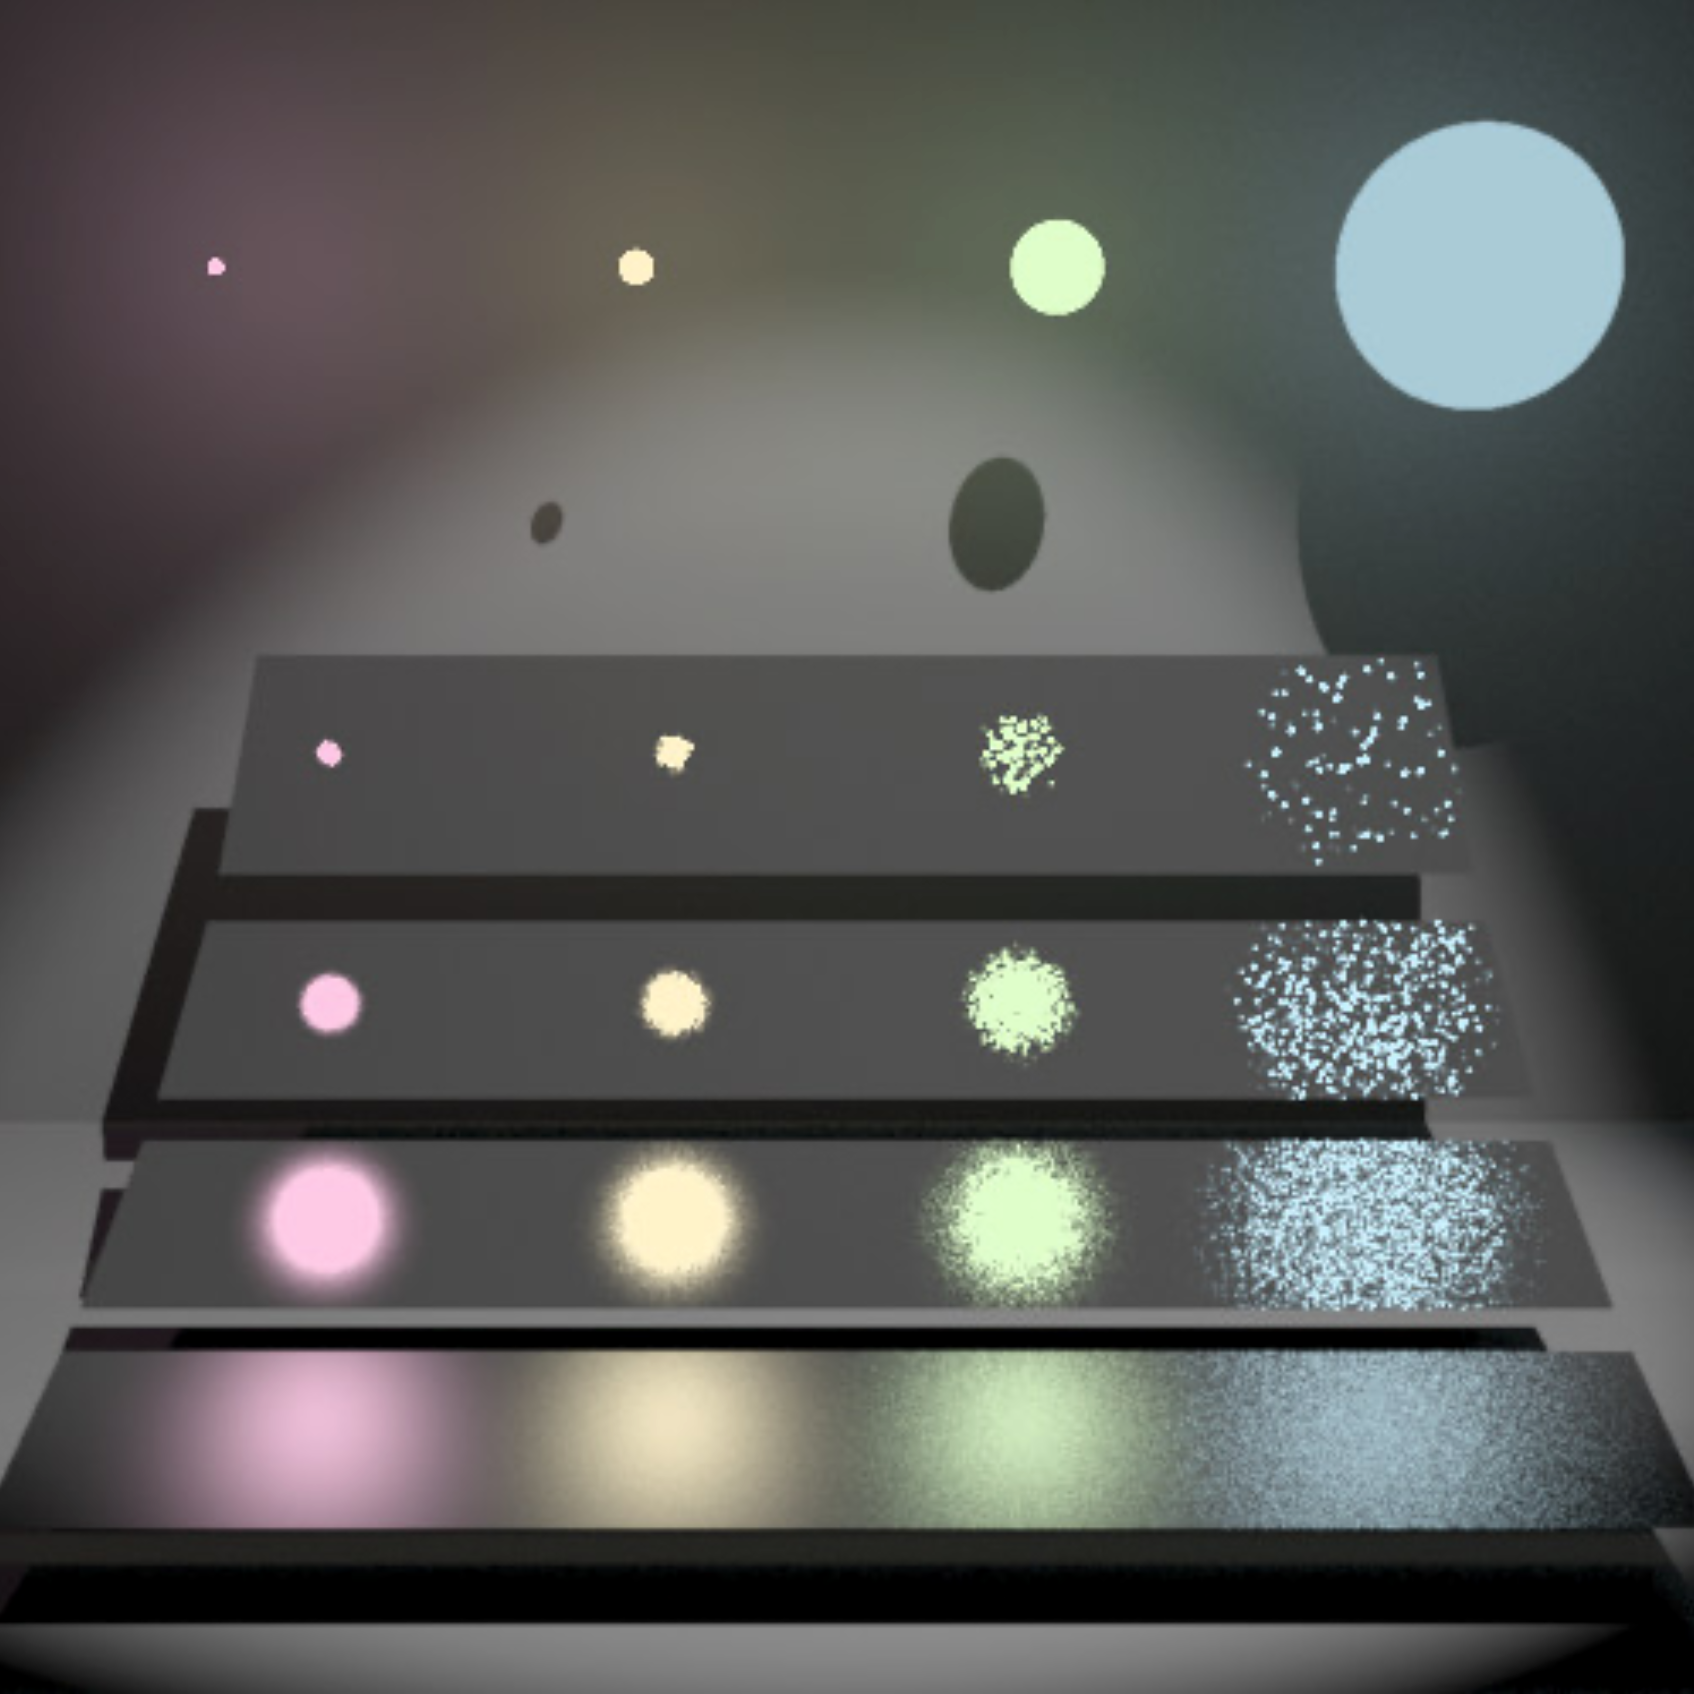
\includegraphics[width=\textwidth]{images/veach_mis_light.png}
        \caption{Sampled after the light sources}
        \label{fig:veach_mis_light}
    \end{subfigure}
    \caption{A scene with four light sources getting larger in diameter from left to right
    and four horizontal objects with BSDFs from diffuse at the bottom to more and more specular at the top.\\
    (a) This scene is sampled using a pdf that is proportional to the BSDF of the surface.\\
    (b) Here the scene was sampled with a pdf that generated samples on the light source.
    These graphics were taken from~\cite[Figure~9.2]{veach-thesis}.}
    \label{fig:veach_mis_single}
\end{figure}

If we could combine both approaches the result should cover all cases and show all reflections well.
To do this Veach introduced Multiple Importance Sampling~\cite[Chapter~9]{veach-thesis}.
The updated estimator now looks like this: $$ F = \sum_{i = 1}^k \frac{1}{n_i} \sum_{j = 1}^{n_i} w_i(X_{i,j}) \frac{f(X_{i,j})}{p(X_{i,j})}. $$
Compared to the initial estimator from equation \ref{eq:monte_carlo_integral} we now have additional weight functions $ w_i(.) $
and split up our samples over the $ k $ different sampling technique with $ n = \sum_{i = 1}^k~n_i $.
To keep the estimator unbiased the weighting function need to fulfill two constraints:
\begin{itemize}
    \item $ \sum_{i = 1}^n w_i(x) = 1 $ when $ f(x) \neq 0 $
    \item $ w_i(x) = 0 $ when $ p_i(x) = 0 $.
\end{itemize}
The first constraint makes sure that every point is neither reduced nor increased in its contribution
which is important to keep the estimator unbiased.
The second constraint states that a pdf that could not create this sample also must have no weight
so it will be ignored.
A concrete weighting function will be introduced in the next subsection.


\subsection{Balance Heuristic}
\label{sec:balance_heuristic}
A very popular weighting function also introduced by Veach is the balance heuristic~\cite[Chapter~9.2.2]{veach-thesis}.
The formula to calculate it is as follows: $$ w_i(x) = \frac{n_i p_i(x)}{\sum_{j = 1}^k n_j p_j(x)} $$
So the weight for a sample consists of the amount of samples $ n_i $ drawn with that technique,
the probability $ p_i(x) $ for that sample divided by the sum of all techniques.
\todo{show how it falls down to a simple standard monte carlo estimator when inserting into the formula (when more text is needed?)}

\begin{figure}[h]
    \centering
    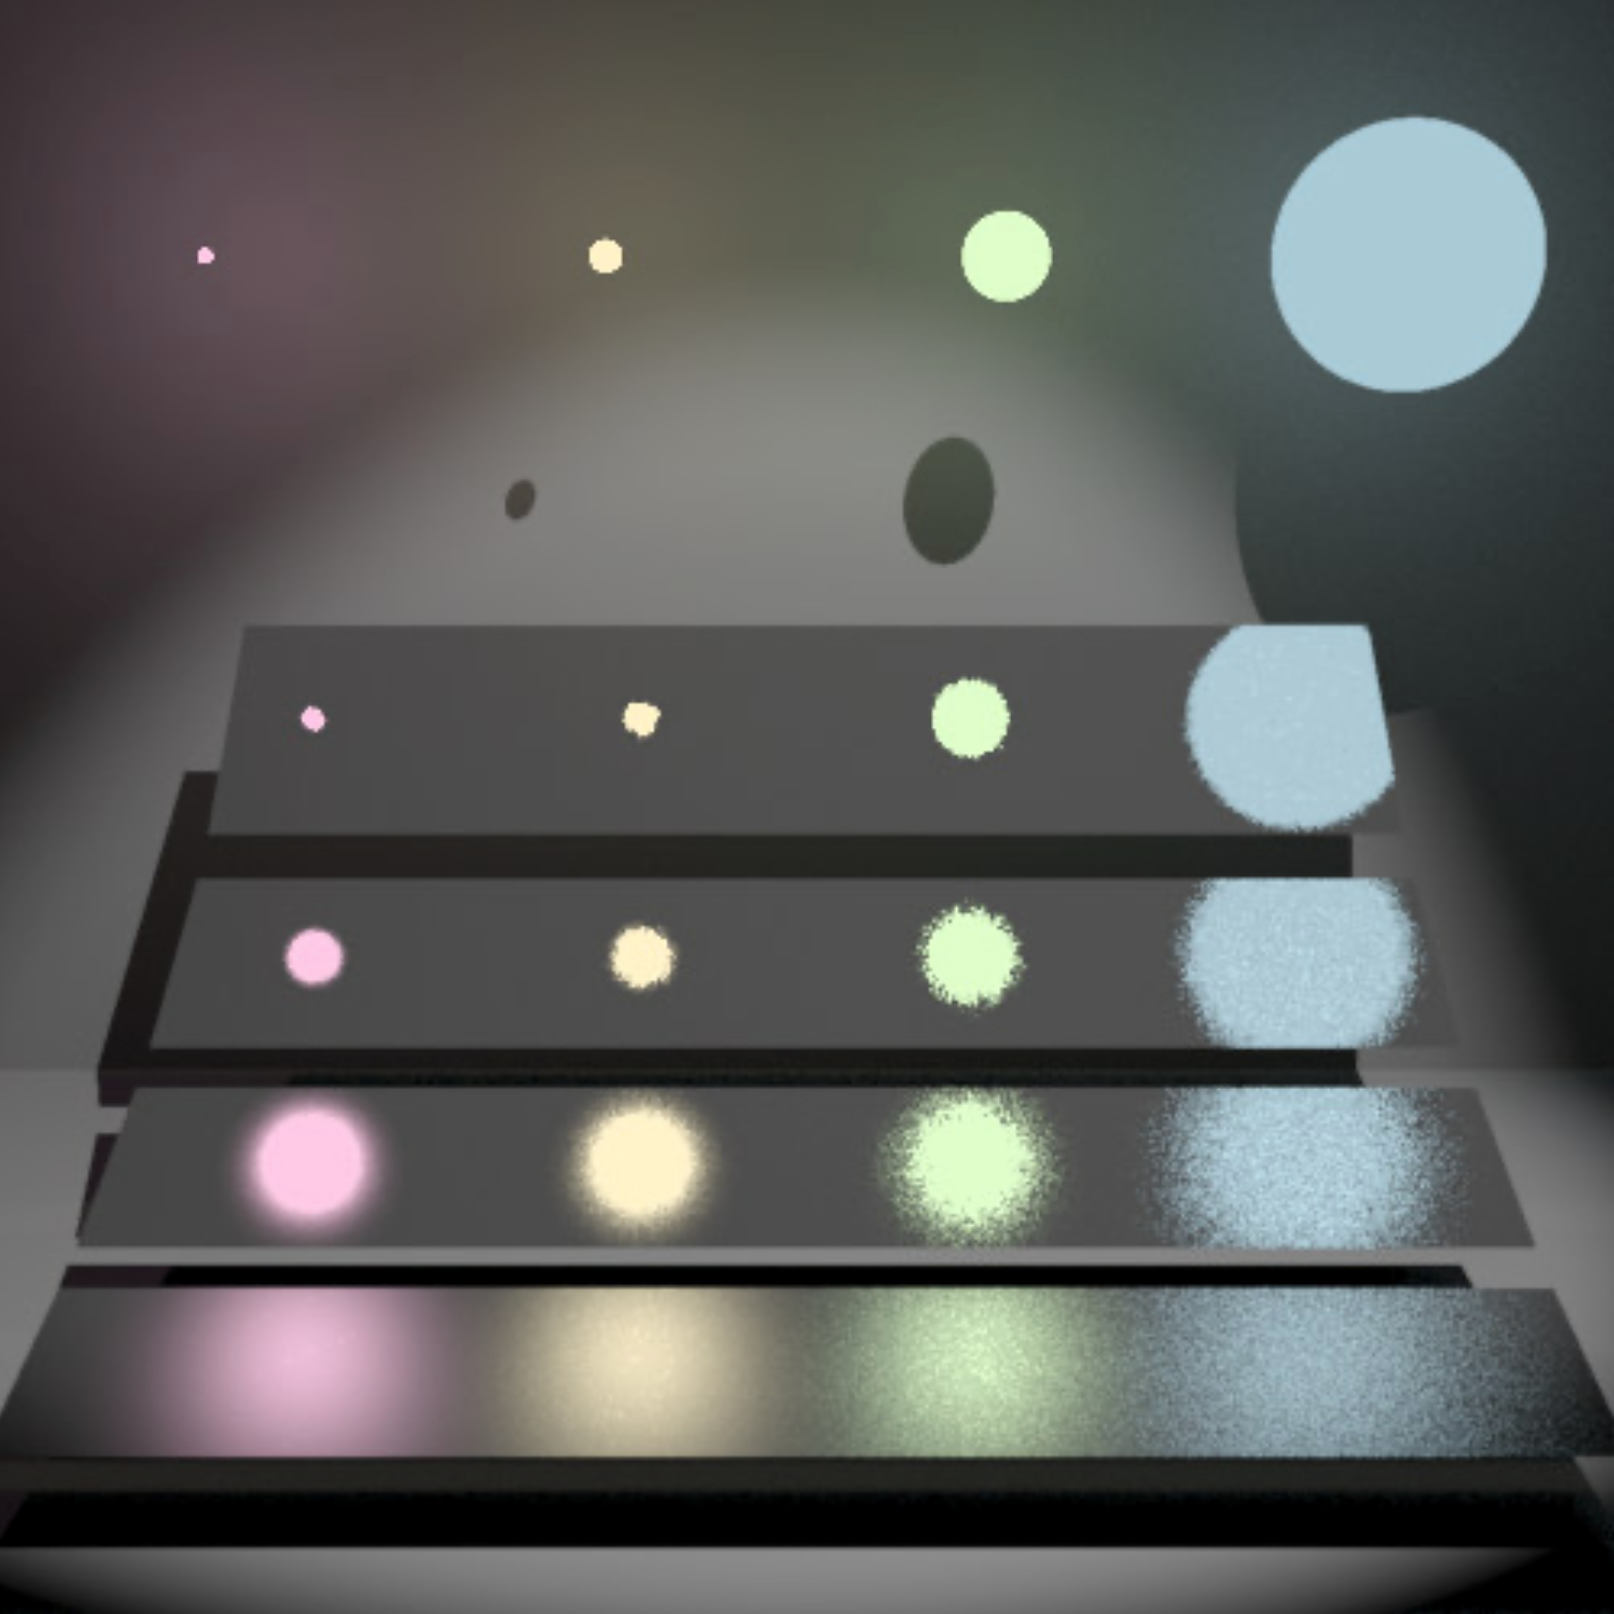
\includegraphics[width=.45\textwidth]{images/veach_mis_both.png}
    \caption{This image shows the same scene as in figure \ref{fig:veach_mis_single} but rendered using the balance heuristic. Taken from~\cite[Figure~9.4]{veach-thesis}.}
    \label{fig:veach_mis_balance}
\end{figure}

Figure \ref{fig:veach_mis_balance} show that with the balance heuristic the noisy areas we observed
while only using a single pdf in figure \ref{fig:veach_mis_single} disappeared
and all combinations of surface roughness and light source size are well represented.
\chapter{Multiple Importance Sampling Compensation}
\label{ch:mis_compensation}
This chapter will cover the theory behind MIS compensation as proposed by Karl\'ik et al. in~\cite{Karlik2019}.
First the basic idea of MIS compensation will be explained after which the variance reduction will be proven.

As we can see in figure~\ref{fig:pdf_comparison} when we use our pdfs regularly with the balance heuristic
the resulting pdf is too defensive as the high values are undersampled and the low values are oversampled.
The name for their techniques comes from the compensation for the averaging of the balance heuristic.
One resulting pdf of their approach can be seen in figure~\ref{fig:optimized_mis}.

\begin{figure}[h]
    \centering
    \begin{subfigure}[b]{.3\textwidth}
        \centering
        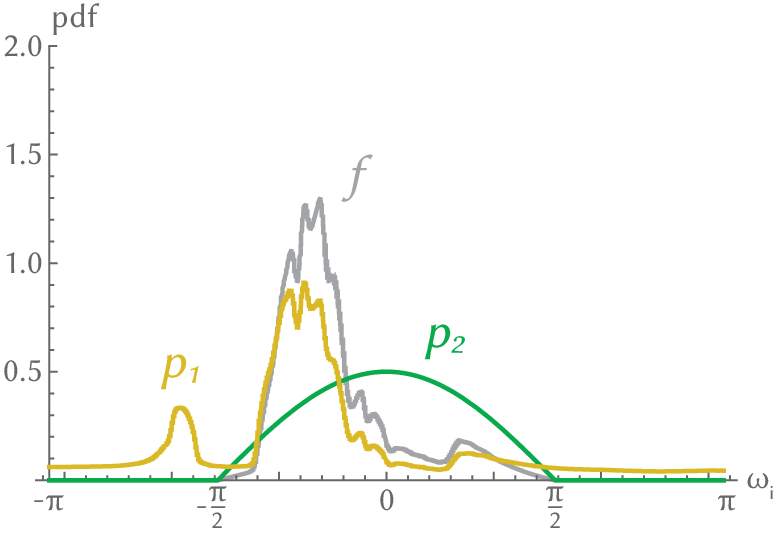
\includegraphics[width=\textwidth]{images/original_setup.png}
        \caption{Original pdfs}
        \label{fig:original_setup}
    \end{subfigure}
    ~
    \begin{subfigure}[b]{.3\textwidth}
        \centering
        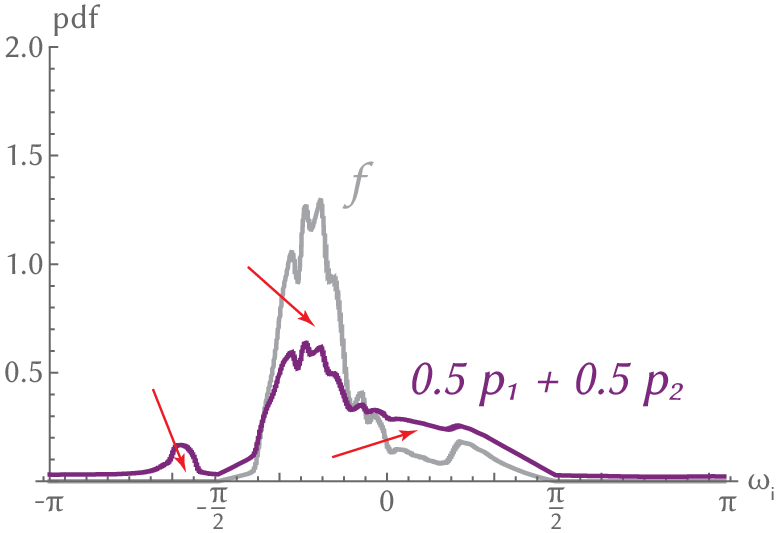
\includegraphics[width=\textwidth]{images/mis_setup.png}
        \caption{Original MIS}
        \label{fig:original_mis}
    \end{subfigure}
    \\
    \begin{subfigure}[b]{.3\textwidth}
        \centering
        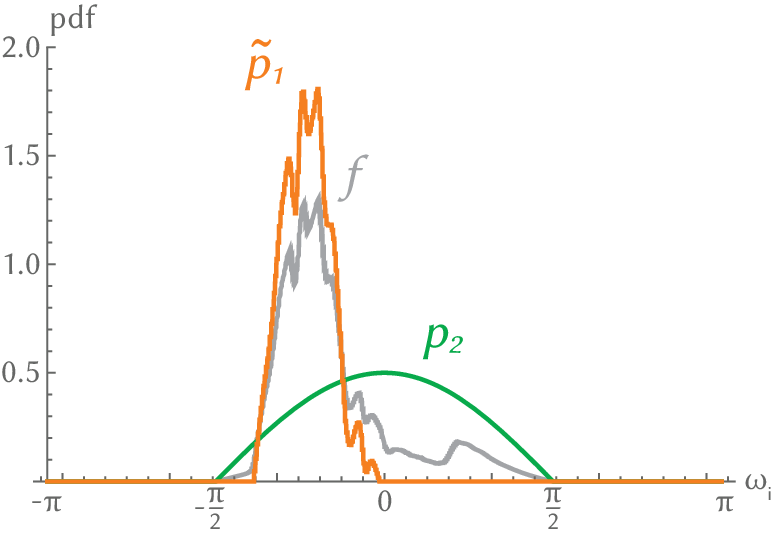
\includegraphics[width=\textwidth]{images/optimized_setup.png}
        \caption{Optimized pdfs
        \label{fig:optimized_setup}}
    \end{subfigure}
    ~
    \begin{subfigure}[b]{.3\textwidth}
        \centering
        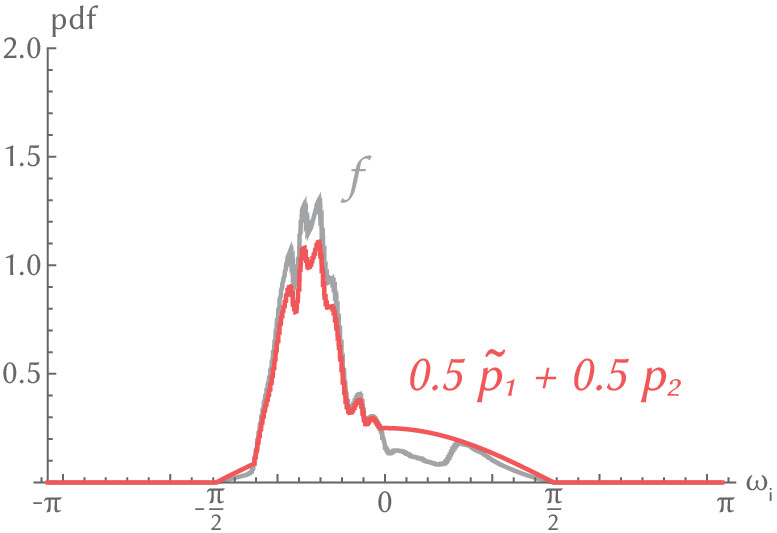
\includegraphics[width=\textwidth]{images/mis_optimized.png}
        \caption{Optimized MIS}
        \label{fig:optimized_mis}
    \end{subfigure}
    \caption{Comparison of the original pdfs without compensation~(\ref{fig:original_setup})
    and how the combined pdf looks like with the balance heuristic~(\ref{fig:original_mis})
    with the modified pdf~(\ref{fig:optimized_setup}) and the balance heuristic using the optimized pdf~(\ref{fig:optimized_mis}).
    f (gray) is the function we want to integrate.
    Figure~\ref{fig:original_mis} shows that the high values are undersampled and the low values are oversampled (see the red arrows).
    The optimized pdfs match the integrand much better when using MIS as seen in figure~\ref{fig:optimized_mis}.
    Figures taken from~\cite[Figure~2]{Karlik2019}.}
    \label{fig:pdf_comparison}
\end{figure}

From a given set of samplers $ T $ they pick one sampler $ t \in T $ and call its pdf $ p_t $ the free pdf that will be used for compensation
so that the combined pdf reduces the variance when used with the balance heuristic.

In an optimal solution the combined pdf $ p_{eff}(x) = f(x)/F $ would lead to zero variance as shown in equation~\ref{eq:zero_variance}.
For the purposes of MIS compensation the combined pdf can also be written as $ p_{eff}(x) = q(x) + c_t p_t(x) $ where $ q(x) = \sum_{i \in T/\{t\}} c_i p_i(x) $
and $ p_t $ is the free pdf with $ c_t $ being its fraction of the total samples.
Whe can reorder to get a formula for
\begin{equation}
    \label{eq:compensated_pdf}
    p_t(x) = \frac{f(x)}{c_t F} - \frac{q(x)}{c_t}.
\end{equation}
This however does not guarantee that $ p_t $ is a valid pdf,
for this they clamped and normalized it and got this formula: $$ \tilde{p}_t(x) = \frac{1}{b} max\{0, p_t(x)\} $$ with a normalization factor of $ b = \int_X max\{0, p_t(x)\} dx $.

Their compensated pdf fills the gap between the other samplers and the target function $ f(x) $
since it effectively samples only the parts that the other samplers missed in regard to $ f(x) $.
Whenever $ f(x) > 0 $ also $ p_{eff}(x) > 0 $ has to hold true for it to be unbiased.
When we assume $ q(x) = 0 $ then $ p_t(x) > 0 $, because of its definition~\ref{eq:compensated_pdf}.
If $ q(x) > 0 $ then $ p_t(x) $ could become $ 0 $, but then still $ p_{eff}(x) > 0 $ would be the case.
So the combined pdf is valid but it doesn't guarantee to reduce variance, because of the max operator and the re-normalization.


\section{Optimality}
\label{sec:misc_optimality}
\todo{Ulala}
write variance as second moment - F2 with second moment being formula and p opt\dots
To avoid max and normalization we set two constraints\dots
Formula from appendix to derive $ \lambda $.
Since we need the max there is no analytical solution to the optimal pdf so it needs to be calculated iteratively which makes it impractical
If the mis-compensated solution (from above in square braces in the paper) is close-enough to the optimal solution, which is often the case that can be used instead

\subsection{Bounds for the MIS-compensated solution}
To show the similarity of the optimal solution and the MIS-compensated one we derive following bounds \dots by \dots (appendix B)
With eq. 9 we can easily see that the optimal and the compensated solution are equal and the lower bound applies. (just input into 9, fulfill conditions)
with this we can assume that the optimal solution is often not far from the compensated one.
In case they are not the same we want to see how badly using the compensated pdf over the optimal one can increase variance
the highest increase would be 1 / ct over the optimal solution.
to get a concrete number for the introduced variance multiple scenes were tested with the worst result being 1.6 times

They showed that the compensated pdf is often similar to the optimal one.
In case they are not the same it is expensive to calculate the optimal pdf since it involves iteratively evaluating the integral and checking if the conditions hold true
the mis-compensated solution can be used because it is easy to calculate with an approximation of F and is still a good overall solution.

\todo{is it okay to refer to the original paper for the derivation of the optimal solution (appendix proovs)}

\todo{show how F will be approximated by $\lambda$. maybe no approach to approximation is shown}

\todo{Explain their work. Formulas should be clearly explained.}
\chapter{Application: Image-Based Lighting}
\label{ch:application_ibl}


\section{Image-Based Lighting}
\label{sec:ibl}
Creating realistic lighting for a scene can be very complex and time consuming.
To avoid modelling a lighting environment a commonly used method is to create an image of a real world environment
and using that for the direct illumination of a scene.
This approach is called image-based lighting and was introduced back in 1998 by Debevec in~\cite{debevec}.\\
To get the lighting of a scene in the real world you could place a mirror sphere in the middle of your scene
and the a photo of that sphere from far away
so the camera itself doesn't take up a large part of the scene.
This method is called sphere mapping.
During rendering you place your scene in the center of that textured sphere
and if a shadow ray doesn't hit any object of the scene you read out the texel
on the sphere that corresponds to the direction of the ray.\\
A different method is to take six pictures of the scene from the top, bottom, left, right, front and back
and then use the same evaluation method as with the sphere with the direction of the shadow ray direction
to get the texel from the environment map.
For more information on how to use environment maps/image-based lighting consider~\cite{environment_map}.


\section{MIS Compensation in Image Based Lighting}
\label{sec:misc_ibl}
Here we will discuss the image-based lighting application example from Karl\'ik et al. in~\cite[Section~6-7]{Karlik2019}.


\subsection{Setup}
\label{sec:ibl_setup}
They calculate the unoccluded direct illumination with the following rendering equation:
\begin{equation}
    \label{eq:ibl_render_equation}
    L_{dir}(x, \omega_o) = \int_{H(n)} L_I(\omega_i) \rho(x, \omega_i, \omega_o) |n \cdot \omega_i|_+ d\omega_i.
\end{equation}
$ x $ is the surface position and $ \omega_o $ the outgoing view direction.
The integration domain $ H(n) $ is the upper hemisphere centered around the normal $ n $.
The HDR environment map is used through $ L_I(w_i) $,
$ \rho(x, \omega_i, \omega_o) $ corresponds to the BRDF at position $ x $
with incoming direction $ \omega_i $ and outgoing direction $ \omega_o $.
$ |n \cdot \omega_i|_+ $ is the positive cosine of the angle between the normal and the incoming direction i.e. $ \max\{0, |n \cdot \omega_i|\} $.\\
In a standard Monte Carlo renderer two pdfs would be used,
one proportional to the BRDF-cosine product and another one proportional to the environment map.
Those two would then be combined in MIS with the balance heuristic.
Generally the BRDF-cosine product pdf is given analytically and depends on the position, the outgoing and the incoming direction
whereas the environment map pdf is mostly tabulated and only depends on the incoming direction.
Since the second one is easier to modify,
that one was used as the free pdf in their work.


\subsection{PDF solutions}
\label{sec:ibl_pdfs}
To get the compensated pdf sampling technique Equation~\ref{eq:ibl_render_equation}
and the BRDF sampling pdf $ p_{\rho}(x, \omega_i, \omega_o) $ are inserted into Equation~\ref{eq:valid_compensated_pdf}
to get $$ \tilde{p}_I(x, \omega_i, \omega_o) = \frac{1}{b} \max\{0, \frac{f_I(x, \omega_i, \omega_o)}{c_I L_{dir}(x, \omega_o)} - \frac{1 - c_I}{c_I} p_\rho(x, \omega_i, \omega_o)\} $$
where $ f_I(x, \omega_i, \omega_o) = L_I(\omega_i) \rho(x, \omega_i, \omega_o) |n \cdot \omega_i|_+ $,
$ c_I $ is the proportion of samples for the free pdf and b is the normalization factor to make it integrate to one.
Since this solution depends on the position, the incoming and the outgoing direction they proposed a simpler solution which we will show in the upcoming section.


\paragraph{Normal-dependent solution}
\label{par:ibl_normal_dependent}
To remove the dependency on the position and the outgoing direction they assumed a Lambertian BRDF with albedo $ \rho \equiv \frac{1}{\pi} $
which yields:
\begin{equation}
    \label{eq:normal_dependent}
    p_I^{nd}(\omega_i, n) = \frac{1}{b_{nd}} \max\{0, \frac{f_{nd}(\omega_i, n)}{c_I \int_{H(n)} f_{nd}(\omega, n) d\omega} - \frac{1 - c_I}{c_I} \frac{|n \cdot \omega_i|_+}{\pi}\}.
\end{equation}
This formula does depend on the surface normal,
but it can still be precomputed for a number of directions.
Since this solution is more practical than the more general one before it still might require changes in the rendering implementation.
Therefore they introduced one more solution that uses less memory and has even less dependencies.


\paragraph{Normal-independent solution}
\label{par:ibl_normal_independent}
This method averages over all normal directions (for a detailed explanation please refer to~\cite[Appendix~D]{Karlik2019})
to get a pdf that is only dependent on the incoming direction: $$ p_I^{ni}(\omega_i) = \frac{1}{b_{ni}} \max\{0, L_I(\omega_i) - 2 (1 - c_I) \bar{L}_I\}. $$
As above $ b_{ni} $ is the normalization factor and $ \bar{L}_I $ is the average of the HDR map luminance.
If we look close we see that the formula corresponds to a simple subtraction from the complete environment map and then re-normalizing it.


\subsection{Evaluation}
\label{sec:ibl_evalution}
They used a simple 1D setup as shown in Figure~\ref{fig:ibl_setup} for their empirical tests.

\begin{figure}[h]
    \centering
    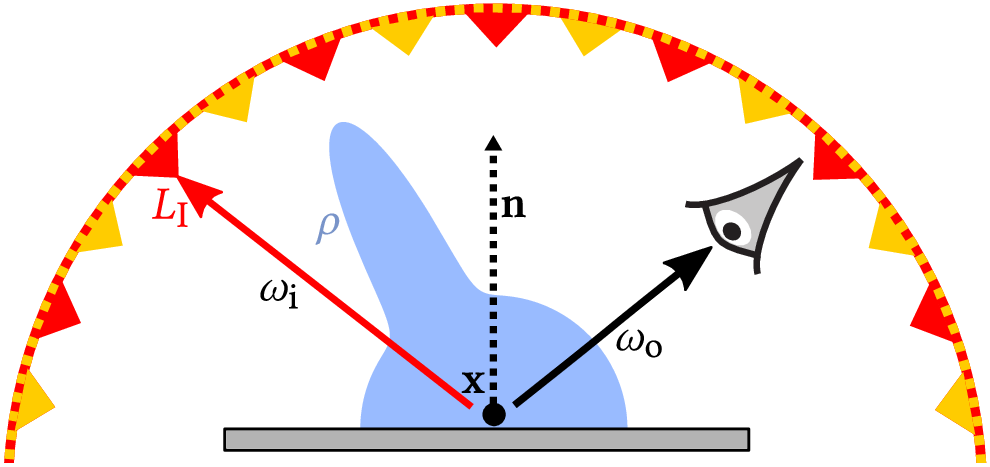
\includegraphics[width=.4\textwidth]{images/ibl_setup.png}
    \caption{Setup for the evaluation of their method.
    \cite[Figure~3]{Karlik2019}}
    \label{fig:ibl_setup}
\end{figure}

The original pdfs seen in Figure~\ref{fig:ibl_pdfs} correspond to the HDR map (in yellow) and the BRDF (in green).

\begin{figure}
    \centering
    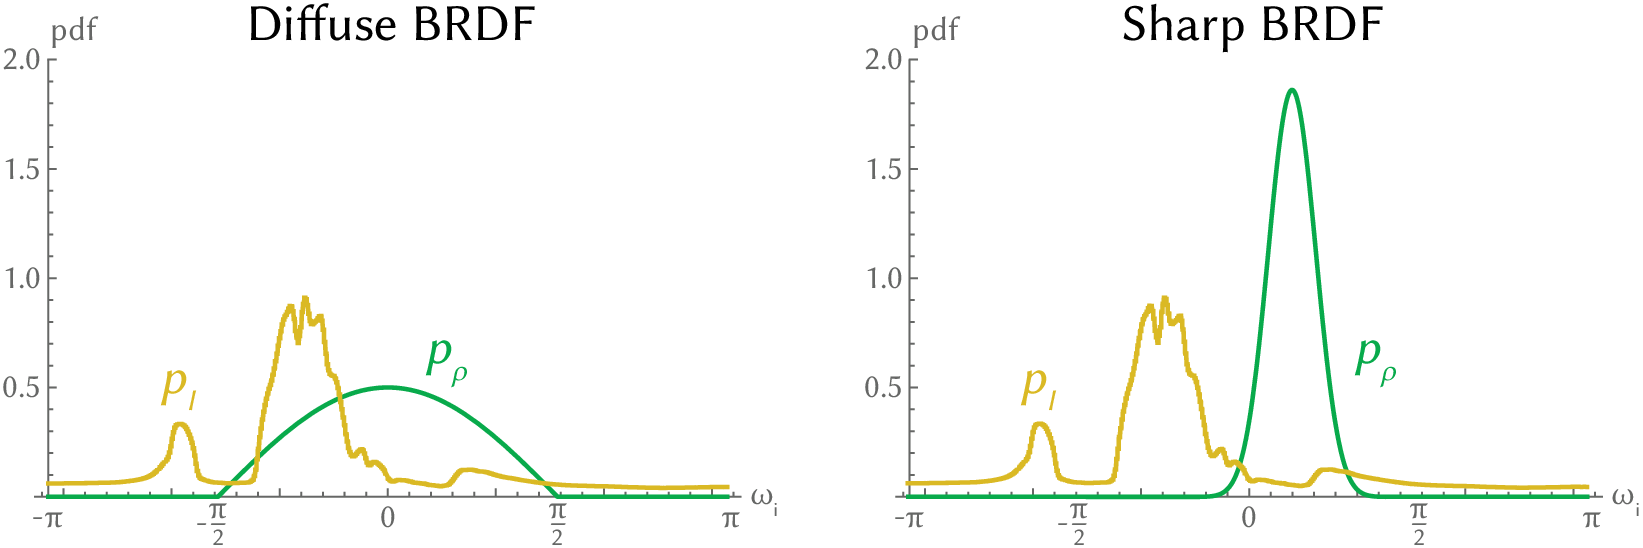
\includegraphics[width=.7\textwidth]{images/ibl_pdfs.png}
    \caption{Original pdfs for the 1D setup.
    The diffuse BRDF corresponds to $ \frac{1}{\pi} $
    whereas the shard BRDF represents a normalized Phong lobe~\cite{phong} with exponent 20 moved by $ \frac{\pi}{8} $ to the right.
    \cite[Figure~4]{Karlik2019}}
    \label{fig:ibl_pdfs}
\end{figure}

In Figure~\ref{fig:compensated_pdfs} the different pdf they proposed are shown
where the Lagrange multiplier $ \lambda $ was calculated with a \enquote{iterative bisection root-finder within 100 iterations}~\cite[Section~6.3]{Karlik2019}.
The MIS-compensated solution and the optimal one are almost identical with a discrepancy no larger than $ 10^{-5} $
for the mean squared error (MSE) as tested by them in different setups.
The practical pdfs only fit well for the diffuse case, because a diffuse BRDF was assumed in their creation.
Note that the normal-dependent and normal-independent solution are almost the same except that the normal-independent one has some values for angles outside of $ [ -\frac{\pi}{2}, \frac{\pi}{2} ] $.

\begin{figure}
    \centering
    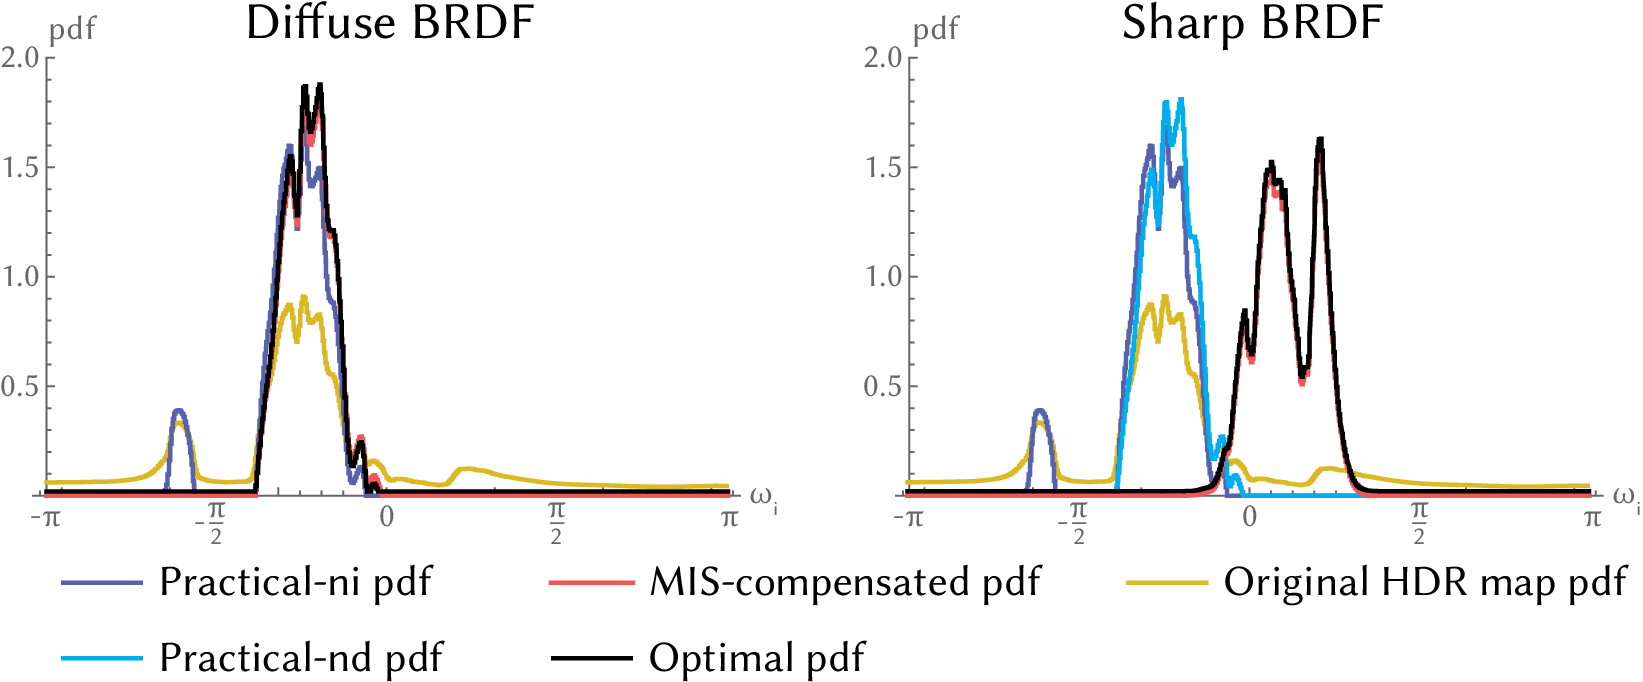
\includegraphics[width=.7\textwidth]{images/ibl_compensated_pdfs.png}
    \caption{Comparison of the different pdfs for the diffuse and sharp BRDF from Figure~\ref{fig:ibl_pdfs}.
    \cite[Figure~5]{Karlik2019}}
    \label{fig:compensated_pdfs}
\end{figure}

Figure~\ref{fig:error_plots} shows the MSE of a one-sample and a multi-sample estimator for the diffuse and sharp BRDFs from Figure~\ref{fig:ibl_pdfs}.
For the diffuse BRDF of the one-sample estimator sampling from the HDR map compared to standard MIS is almost identical.
Their normal-independent solution is 3.7 times better in regards to the MSE.
The normal-dependent, optimal and compensated pdfs improve the MSE by a factor of 7.5.
For the sharp BRDF the MSE is not improved when using one of the practical pdfs but more importantly it also doesn't worsen it which makes it a good choice compared to standard MIS,
but compared to sampling the BRDF it is worse for a sharp BRDF.
When comparing the optimal solution and the compensated pdf with sampling the BRDF we see an improvement in the MSE by 847 times and compared to regular MIS a 4809 times better MSE.
This shows that there is a lot of potential for better approximations of the compensated pdf.

For the multi-sample estimator the results are similar to the one-sample one,
but note the curve of the practical solutions which are now almost as good as sampling the sharp BRDF,
so even in that case the practical solutions are well suited.
Since the balance heuristic is not the optimal solution for the weights in a multi-sample estimator,
also the optimal weights~\cite{Kondapaneni2019} are shown.
Note that there is still a large discrepancy between the optimal weights and the optimal pdf which suggests that there is a lot of potential in finding better pdfs.
The reason why optimal weights can't compete with an optimal pdf is, because no linear combination of the available pdfs is good approximation of the integrand.

\begin{figure}
    \centering
    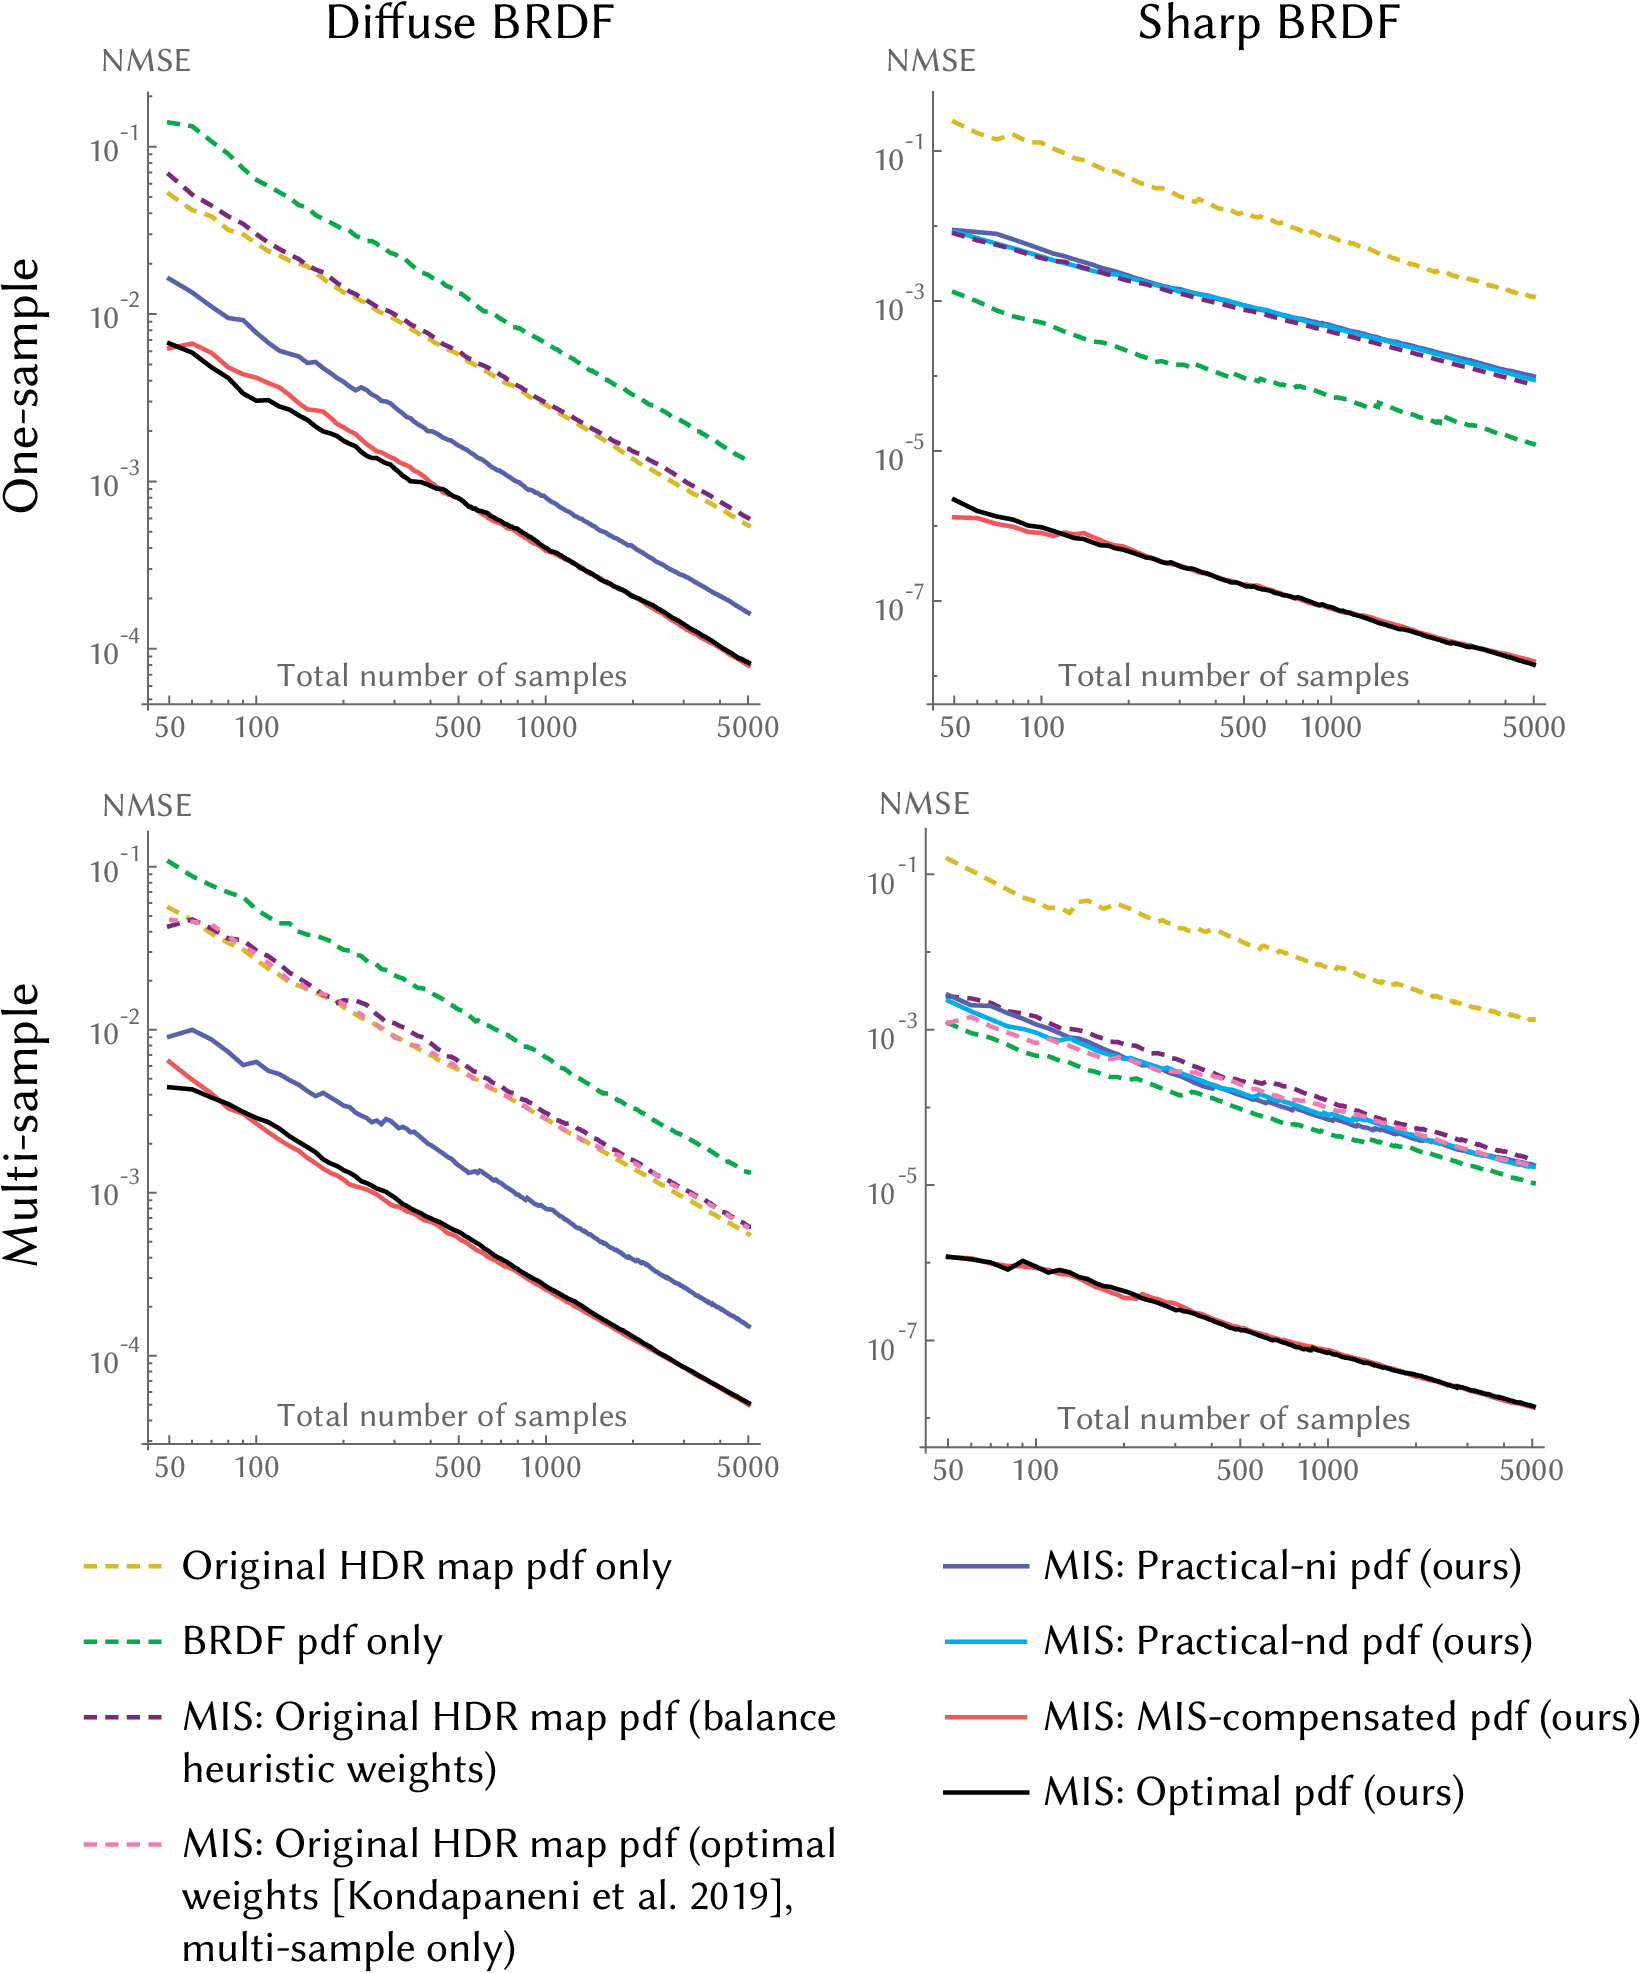
\includegraphics[width=.7\textwidth]{images/error_plots.png}
    \caption{Log-log normalized plot of the MSE for the different estimators.
    The top row shows the results from a one-sample estimator where the bottom row shows the MSE of a multi-sample one.
    In the top row only the balance heuristic is shown as it is provably optimal
    and in the bottom row also the optimal MIS weights from~\cite{Kondapaneni2019} are shown.
    \cite[Figure~6]{Karlik2019}}
    \label{fig:error_plots}
\end{figure}

They also did some experiments with real and synthetic scenes to verify their results as can be seen in Figure~\ref{fig:sphere_comparison} and~\ref{fig:pills}.
We can see that the variance improvements vanish the lower the contrast of the HDR map becomes and the more specular the object is.
In the Pills scene~\ref{fig:pills} we can clearly see that the compensation reduced the variance noticeably.

\begin{figure}
    \centering
    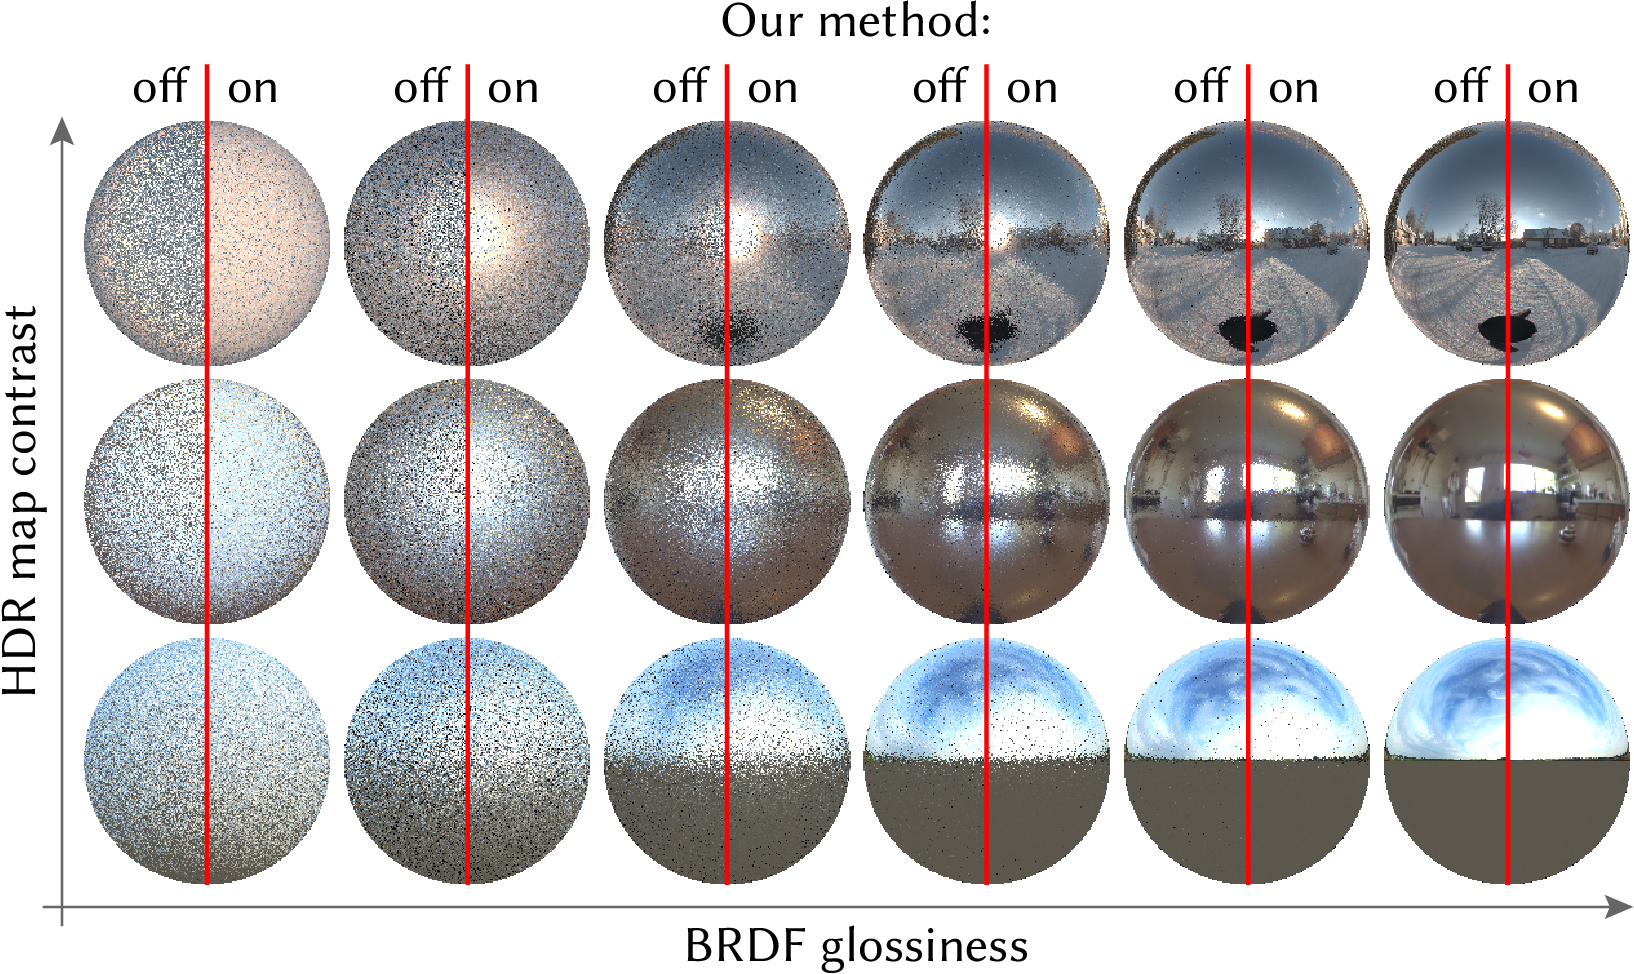
\includegraphics[width=.6\textwidth]{images/sphere_comparison.png}
    \caption{One sample per pixel comparison of rendered spheres with increasing glossiness (from left to right) and HDR map contrast (from bottom to top).
    The left half is rendered with standard MIS and the right half with their normal-independent method.
    \cite[Figure~7]{Karlik2019}}
    \label{fig:sphere_comparison}
\end{figure}

\begin{figure}
    \centering
    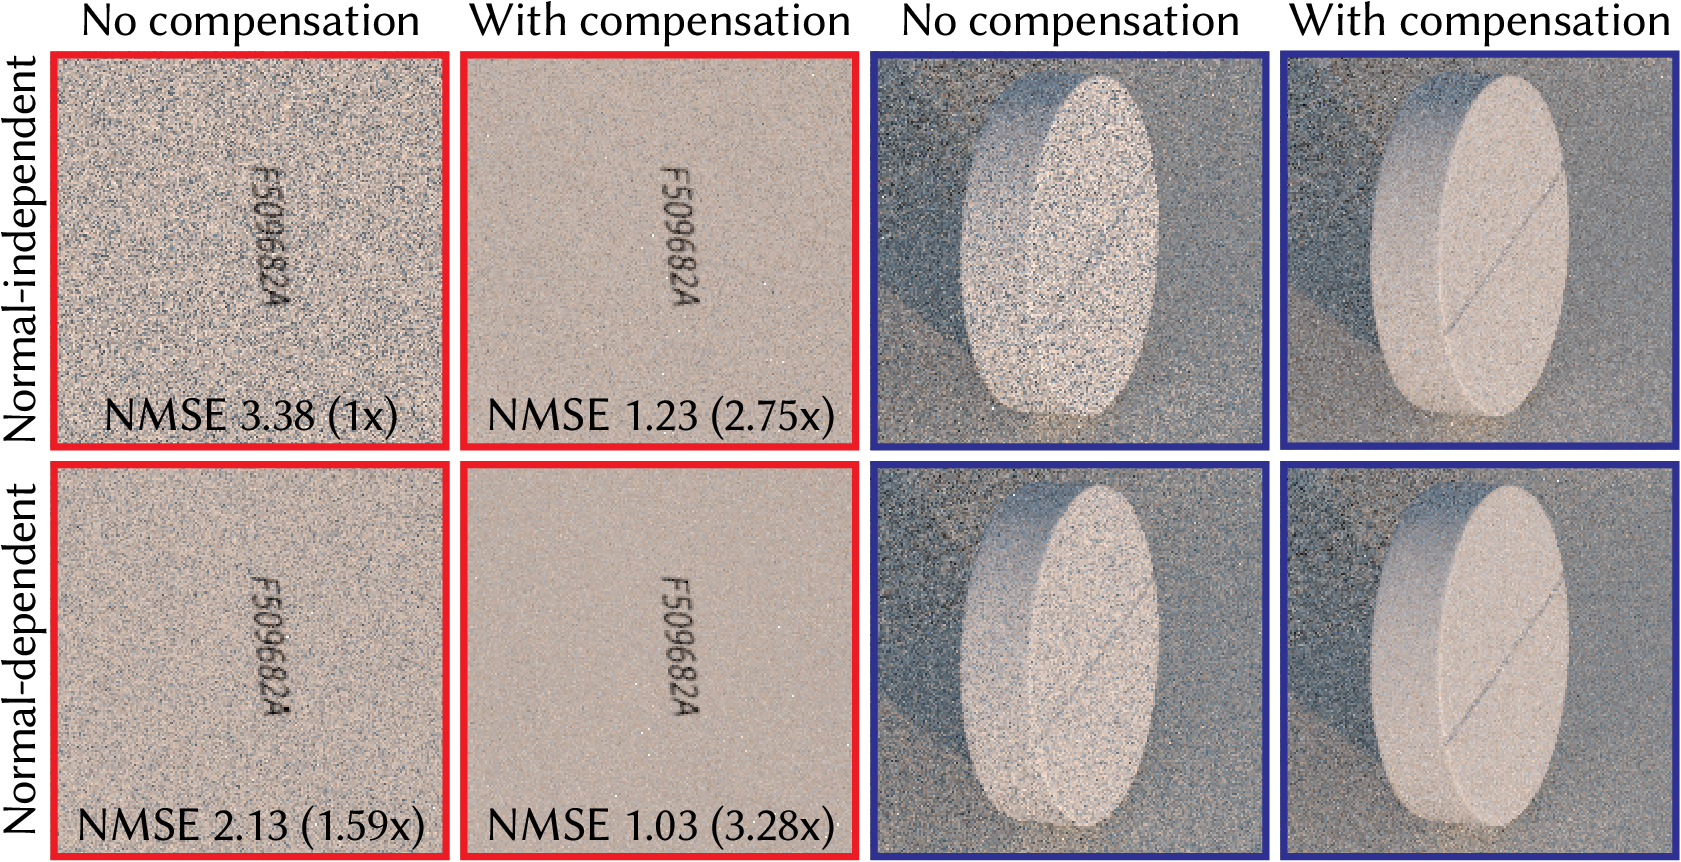
\includegraphics[width=.6\textwidth]{images/pills.png}
    \caption{Equal-time (5s) render of the Pills scene to compare the effect of using MIS compensation with and without normal dependency.
    The normal-independent uncompensated solution show regular MIS
    whereas the normal-dependent uncompensated render shows the effect of premultiplying the HDR map with a diffuse BRDF for each normal direction
    which corresponds to evaluating Equation~\ref{eq:normal_dependent} without the subtraction.
    \cite[Figure~9]{Karlik2019}}
    \label{fig:pills}
\end{figure}
\chapter{Application: Path Guiding}
\label{ch:application_pg}

\section{Path Guiding}
\label{sec:path_guiding}
\todo{Explain the concept of path guiding}

\section{MIS Compensation in Path Guiding}
\label{sec:misc_path_guiding}
\todo{Explain how their approach improves path guiding}
\chapter{Conclusion}
\label{ch:conclusion}
Karl\'ik et al.~\cite{Karlik2019} extended the options for variance reduction in the MIS domain
by introducing a technique to modify one of the sampling densities to better fit the integrand.
They derived a MIS compensated pdf from the standard balance heuristic in an MIS setup to reduce variance.
A practical and simpler pdf was presented for use in current renderers
and also an optimal pdf that is difficult to create but shows what is possible.
Examples in image-based lighting and path guiding were shown,
where the advantage in IBL is much more substantial than in path guiding,
but they could still improve both applications of MIS.


\paragraph{Future Work}
\label{par:future_work}
\textit{Specular BRDF} Karl\'ik et al.~\cite{Karlik2019} used a diffuse BRDF for their approximations
and therefore the results excel when working with diffuse surfaces,
but don't aid much when the BRDF becomes more specular.
Therefore approximations that incorporate the BRDF could further reduce variance.

\textit{Image-based lighting} In IBL they used unoccluded illumination which already improved the results a lot,
but taking occlusion into account could further reduce variance.

\textit{Combining compensation and sample distribution} In their tests they used equal samples among all pdfs.
Combining their approach with also optimally distributing samples over the used pdfs could additionally help with variance reduction.




%% --------------------
%% |   Bibliography   |
%% --------------------
\cleardoublepage
\phantomsection
\addcontentsline{toc}{chapter}{\bibname}

\iflanguage{english}
{\bibliographystyle{IEEEtranSA}}	% english style
{\bibliographystyle{babalpha-fl}}	% german style

% Use IEEEtran for numeric references
%\bibliographystyle{IEEEtranSA})

\bibliography{ausarbeitung}
\Erklaerung
\end{document}
